\documentclass[oneside,a4paper,10pts,article]{memoir}

\usepackage{palatino}
\usepackage{graphicx}
\usepackage{todonotes}
\presetkeys{todonotes}{inline}{}

\usepackage{url}
\usepackage[hidelinks,hyperindex]{hyperref}

\captionnamefont{\bfseries}

\usepackage{tikz}
\usetikzlibrary{positioning,arrows}

\usepackage{listings}
\lstdefinelanguage{Solidity}{
  alsoletter={.},
  morekeywords={contract, function, modifier, this, new, struct, mapping,
                if, then, else, throw, return, true, false, delete,
                storage, memory, constant, internal, protected, private, public,
                address, int, uint, uint128, uint256, bool, string,
                bytes, bytes1, bytes2, bytes4, bytes8, bytes16, bytes32,
                msg.sender, msg.value, now, msg.gas, msg.data, msg.sig, tx.gasprice
                tx.origin, block.coinbase, block.difficulty, block.gaslimit,
                block.number, block.timestamp, block.blockhash},
  sensitive=true,
  morecomment=[l]{//},
  morecomment=[s]{/*}{*/},
  morestring=[b]",
}
\lstset{
  basicstyle=\ttfamily\footnotesize,
  keywordstyle=\bfseries,
  captionpos=b,
  language=Solidity
}



\title{Trading Certificates of Title as Smart Properties on a blockchain \\
  {\normalfont\normalsize\scshape A case study on a trust-free vehicle
    registry using Ethereum} } \author{Martin Dybdal \\
  \texttt{dybber@dybber.dk}} \date{\today}

\begin{document}

\maketitle

\chapter{Preface}
This report was written as part of the ``Blockchain Summer School
2016'', which was held at the IT University of Copenhagen, August
2016. The summer school concluded with a 1-day hackathon, where we
were assigned a case, that we should solve using blockchain
technology. Group-members: Felix Albert, Jacob Cholewa, Arun Prasad,
Benedikt Notheisen and Martin Dybdal.

\chapter{Introduction}
Blockchain technology is said to revolutionise businesses and public
sector institutions in domains such as finance, logistics and
administration, through the potential digitisation of contracts,
certificates and other legal or financial documents. Blockchain
technology provides a decentralised database infrastructure which is
tamper-proof and trust-free. In essence, a blockchain is a
distributed, append-only digital ledger, which can be trusted, as
consensus on transactions are reached across all nodes in the network
and is made tamper-proof by the use of hashing algorithms. Blockchain
systems are called trust-free, as you do not need to trust any
individual parties; the trust is generated by construction. The
underlying principles and technology behind blockchains is described
in detail in Section \ref{sec:blockchain}.

In this project we have worked on a case arising in public sector
administration, from the Danish Tax Agency (SKAT). SKAT is responsible
for administering the registry of motorised vehicles in Denmark. The
Motor Registry is concerned with most aspects of a cars life cycle,
its initial registration on import, registration and ownership
taxation, insurance, police reports, MOT Tests, repairs and change of
ownership. The current system faces several problems related to lack
of documentation, imbalance of knowledge between parties and imbalance
of trust. It is SKATs hope that a blockchain solution might mitigate
some of these issues, which in turn might reduce the administrative
burden of operating the Motor Registry.

The aspect of ownership change is a core problem in the digitisation
of \textit{Vehicle Titles} (dan. registreringsattester), as there is
an imbalance of knowledge and trust between the buyer and seller. Such
ownership certificates are called \textit{smart properties} when
implemented using blockchain technology
\cite{bitcoinwiki-smartprop}. We have developed a small prototype,
which can represent any such smart property as a tradeable contract on
the blockchain system Ethereum, not just Vehicle Titles. Though not
implemented, we expect that our prototype can be extended to also
address the remaining issues, for instance giving the buyer knowledge
of previous repairs and accidents.

In addition to the specific case, SKAT was interested in understanding
the core technology, to be able to follow the changes it will have on
private industries. In their presentation of the case they were
questioning when private blockchains is suitable, which kind of
consensus mechanism to use, and so on.

The rest of the report is structured as follows. In Section
\ref{sec:blockchain} we will describe Blockchains from a technical
perspective, which is necessary to answer some of the more technical
questions from SKAT. In Section \ref{sec:case} we will introduce the
case from SKAT, and detail the major steps in Vehicle registration and
taxation in Denmark. In Section \ref{sec:trading} we describe the core
problems of trading contracts between two parties, and how these
problems can be solved using a blockchain. In Section
\ref{sec:currency} we look at the problem of representing non-crypto
currencies, such as Danish Kroner or Euro's in a blockchain. In
Section \ref{sec:implementation} we describe our Ethereum prototype
and in Section \ref{sec:futurework} and \ref{sec:conclusion} we
describe future prospects and conclude.

\chapter{Blockchain}
\label{sec:blockchain}
Blockchain technology originates from the technology behind the
Bitcoin crypto-currency \cite{bitcoin}, where it is used to avoid the
problem of double-spending in decentralised transaction
systems. Previously, double-spending was hindered by using a trusted
third party, which verified and timestamped all transactions.

A blockchain is a series of timestamped data blocks, where each block
in the series contains a hash of the previous block. These hashes
serves the purpose of linking the blocks into a chain, such that no
block in the chain can be tampered with, without also updating all
blocks following it.

\begin{figure}[!h]
  \centering
\begin{tikzpicture}
    [remember picture, node distance=5mm and 5mm, ] \footnotesize
    \node[draw] (block1) at (0,0) {
      \begin{tikzpicture}
        \node[anchor=west] (b1title) {Block $n$}; \node[draw, below=of
        b1title.west, anchor=west] (b1prevhash)
        {$\textsf{Hash}(\textrm{Block}~n-1)$}; \node[draw, minimum
        width=3cm, below=of b1prevhash.west, anchor=west] (b1data)
        {Transactions};
      \end{tikzpicture}
    }; \node[draw, xshift=2cm] (block2) at (block1.east) {
      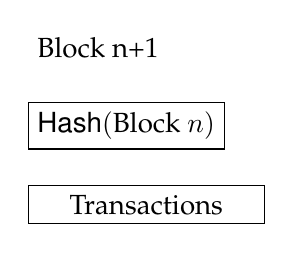
\begin{tikzpicture}
        \node[anchor=west] (b2title) {Block n+1}; \node[draw, below=of
        b2title.west, anchor=west] (b2prevhash)
        {$\textsf{Hash}(\textrm{Block}~n)$}; \node[draw, below=of
        b2prevhash.west, anchor=west, minimum width=3cm] (b2data)
        {Transactions};
      \end{tikzpicture}
    }; \node[draw, xshift=2cm] (block3) at (block2.east) {
      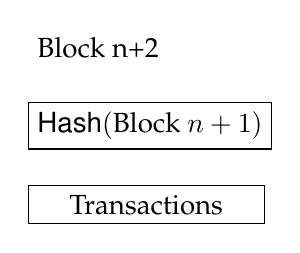
\begin{tikzpicture}
        \node[anchor=west] (b3title) {Block n+2}; \node[draw, below=of
        b3title.west, anchor=west] (b3prevhash)
        {$\textsf{Hash}(\textrm{Block}~n+1)$}; \node[draw, below=of
        b3prevhash.west, anchor=west, minimum width=3cm] (b3data)
        {Transactions};
      \end{tikzpicture}
    }; \node[xshift=-7mm] (block0) at (block1.west) { }; \draw[->]
    (block0.east) -- (b1prevhash); \draw[->] (block1.east) --
    (b2prevhash); \draw[->] (block2.east) -- (b3prevhash);
  \end{tikzpicture}
\end{figure}

Each block contain a package of transactions, with each transaction
signed using public-key cryptography. When a new block is added to the
chain, \textit{all} nodes verify the correctness of the
transactions. That is, checking against double spending and that
agents only spend their own assets.

\section{Reaching consensus}
To ensure that only one linear chain of blocks are allowed, and that
all parties agree on the same course of events, blockchains employ a
consensus mechanism. Such a consensus mechanism is essential to make
double-spending impossible without a third party. 

Essentially what is needed, is that a majority of the nodes in the
distributed network agrees on the same course of events. One might
attempt doing this by a majority vote, where each user has one vote
(e.g. one IP-address one vote). This will however not work. One user
may be able to gather many votes (e.g. many IP-addresses). The vote
has to decided by other means than a simple count.

\subsection{Consensus by Proof-of-Work}
In the original Bitcoin system and in most current blockchain systems,
reaching consensus on a single history of transactions is done by
voting using CPU-power, where nodes have to solve a computationally
hard challenge, to add a new block of transactions to the chain. The
approach is called Proof-of-Work (PoW), and before Bitcoin it was suggested
as an approach to combat spam emails \cite{dwork1992pricing}.

To exemplify, consider the system employed by Bitcoin. An additional
field is added to the block and the nodes have to find a specific
value for this field, such that the entire block's hash has a certain
number of leading zero bits. The difficulty increases exponentially in
the number of zero bits, and difficulty can thus be adjusted over
time. The verification process is cheap however, as it only amounts to
do a hash over a single block.

When a node finds a solution for a block, he broadcasts the new block
to all other nodes, which verify his solution. To accept the solution,
they start working on a solution for the next block. In the case that
several alternative blocks emerge at the same time, nodes will accept
the block they received first. This makes the chain fork in two, which
will resolved by a rule stating that the longest chain wins. At some
point a new block will be added making one of the forks the longest,
at which point the nodes will accept this as the new head, discarding
the all shorter forks.

If an attacker wants to add fraudulent transactions to the chain, he
will have to control more than 50\% of the CPU-power in the network,
otherwise the majority will solve and verify other blocks before him.

\subsection{Consensus by Proof-of-Space}
A major problem with the Proof-of-work system, is the amount of energy
such a scheme will consume. Several alternative consensus mechanisms
has been suggested, to address the energy efficiency of the
Proof-of-Work scheme. One such scheme is \emph{Proof-of-Space}
\cite{dziembowski2015proofs}, where nodes instead will vote using disk
space. In such schemes, all nodes store a large data structure
locally. The challenge used for voting is then not computational like
in Proof-of-Work, but instead done by performing disk-lookups. If the
node can answer on random challenges about what element is located at
different positions in the data structure, proof of space can verified.

Such a scheme does not incur the same energy overhead as
Proof-of-work, as the main part of the work in Proof-of-Space schemes
can be done only once, while generating the data structure, and not
upon each new transcation block. Also, as the original authors claim,
users often have significant amounts of free space, and for such
users, taking part in a Proof-of-Space run blockchain is almost free
\cite{dziembowski2015proofs}. We are not aware of any blockchain
implementations using Proof-of-Space.

\subsection{Consensus by Proof-of-bandwidth}
Another alternative is a scheme, where the nodes votes by transferring
content through a data-network. E.g. handling ordinary data traffic in
the network. The more data you can transfer, the more voting
power. This scheme is called Proof-of-bandwidth and was originally
suggested for the Tor-network \cite{ghosh2014torpath}. Nodes can not
be trusted to report correct bandwidth contributions, thus a
trust-free system for bandwidth measurement is necessary. A
distributed algorithm for doing so is EigenSpeed
\cite{snader2009eigenspeed}.

\subsection{Consensus by Proof-of-Stake}
The final alternative we will mention distributes voting power
relative to the amount of wealth of the nodes (and for how long they
have had the acquired wealth). This consensus scheme is called
Proof-of-Stake, and originates from the Bitcoin-alternative called
Peercoin or PPCoin \cite{king2012ppcoin}.

It has been suggested that Bitcoin moves to a Proof-of-Stake scheme.
Proof-of-Stake has however been criticised for its inability to hinder
long-range attacks. In the Proof-of-Work scheme, it is virtually
impossible to suggest changes to more than one or two blocks behind
the current head, because of the enormous computing power
necessary. In Proof-of-Stake however, attackers can start at any point
in in the entire history of the blockchain, if they were wealthy
enough at that point in time \cite{buterin2014onstake}. In that sense,
Proof-of-Stake is not trustless, you especially have to trust that the
nodes participating in the genesis of the chain will not create an
entire different history of events.

Another criticism is that individual nodes have
\textit{nothing-at-stake}, in the sense that nodes have nothing to
lose from voting on (approving) many different blockchain
histories. When the incentive is lacking for working on only the
longest chain, the vote might never be resolved.

\subsection{Checkpointing}
To resolve the problems of history-rewriting in Proof-of-Stake,
checkpointing has been suggested, with no blockchain reorganization
allowed deeper than the last known checkpoint. Even though the
Proof-of-Work scheme force strong protection, Bitcoin introduced
checkpoints in 2010 \cite{king2012ppcoin}. Using checkpoints also has
the positive impacts that clients joining the network late, do only
need to download the part of the chain from the last checkpoint and
forward, unless they want to verify the entire history of events.

Checkpointing in both Peercoin and Bitcoin is implemented using a
centralized mechanism. In Bitcoin every release of Bitcoin software
contains a new checkpoint. In Peercoin checkpoints are signed using
the Peercoin developer's private key and broadcasted.

% \section{Consistency, availability and partition tolerance}
% As per the CAP Theorem, no system can be both consistent, available
% and partition tolerant.

% \begin{itemize}
% \item ``Impossibility of Distributed Consensus with One Faulty Process''
% \item Byzantine Generals' Problem
% \item Partition tolerancy and CAP Theorem
% \item Privacy and anonymity
% \end{itemize}

\section{Mining incentive}
Every blockchain architecture needs an incentive to mine, such that it
pays off to mine according to the rules. In Bitcoin the miner
successfully adding a block receives a reward of 25 bitcoins. In
addition, each user can pay a transaction fee, and the miner also
collects these transaction fees from the transaction in the current
block. It is voluntary to pay transaction fees, but at the same time
the miner can prioritize incoming transactions and are free to ignore
transactions with low fees.

\section{Ethereum}
Several alternatives to Bitcoin has been proposed. Namecoin was the
first fork of the Bitcoin software and allows users to record and
transfer ownership in a decentralized key/value database
\cite{namecoin}. Namecoin is for instance used to manage the domain
name registry for \texttt{.bit} domains. In this way Namecoin is
implementing a kind of \textit{smart properties}.

Ethereum generalizes the many Bitcoin alternatives to allow any type
of contract to be managed. This allows users to create their own
coins, their own key/value databases and so on, all executing on the
same tamper-proof decentralized blockchain \cite{buterin2013ethereum,
  wood2014ethereum}. We will use the rest of this section to describe
the Ethereum platform.

Ethereum transactions are not restricted to currency-transfer as in
Bitcoin, instead transactions contain general computations in a Turing
complete instruction set, and adds a global updateable state which can
contain any data. This in effect makes the nodes of the Ethereum
network agree on the execution of a sequence instructions. The
instructions executed by a transaction can perform any computation and
update the current state. To verify transactions, all nodes must
execute the issued instructions and check that the invoking
Ethereum-account has permission to perform the operations it requests.

\subsection{Ether and gas}
Like other blockchain solutions, nodes are rewarded for mining. In
Ethereum the reward is payed in a currency called Ether. In addition
as serving as incentive for mining, Ether also serves another
purpose. With a Turing complete language comes the potential of
infinite computations. To avoid malicious users from overloading the
nodes doing expensive computations, users are required to pay for each
instruction executed. The cost thus depends on the size transaction.

However, just like Bitcoin, the transaction fee (gas price) is
voluntary. If you are more eager to get your transaction accepted, you
will set a higher gas price for your transaction. The miners are
allowed to ignore it if the price is set too low.

This limits users from denial of service attacks from infinite loops
and encourages users to write efficient code.

\newpage
\chapter{Case description}
\label{sec:case}
We will now describe the case presented by SKAT on the Danish Motor
Registry. Registration of vehicles, collecting vehicle taxes, and
interacting with other stakeholders, such as police, insurance
companies and transport authorities, requires a lot of administration,
and a lot of things can go wrong in process.

\section{The life cycle of a vehicle}
During the life cycle of vehicle, it goes through various owners and
activities, and involves several different parties, such as car
importers, police, insurance companies, MOT testing centers and
transport authorities. When a car is imported into the country, it is
registered as owned by the importer, which sells it to a specific
dealer. The dealer then sells it to a private owner or a corporation,
and the car can be re-sold multiple times. See Figure \ref{fig:lifecycle}.

A crucial aspect is the change of ownership through the supply chain
and between private persons. Especially the current process of private
car trade is problematic, as there is an imbalance of knowledge and
trust between the seller and the buyer. The buyer might not know the
full history of owners, accidents or repairs, and as the Vehicle Title
is currently on paper, it might be forged or the car might be
stolen. On the other hand, the seller has to put trust in the buyer,
that he will in fact re-register the car in his own name. Currently,
if the buyer does not immediately re-register the car, the sellers
insurance might still be covering damages and the buyer could use the
criminal activities, without being recorded as the owner of the car.

This means that activities such as MOT test, repairs and accident
reports are crucial for the buyer, and for the seller the
re-registration should be a part of the shift of ownership.

\begin{figure} %[b]
  \centering
  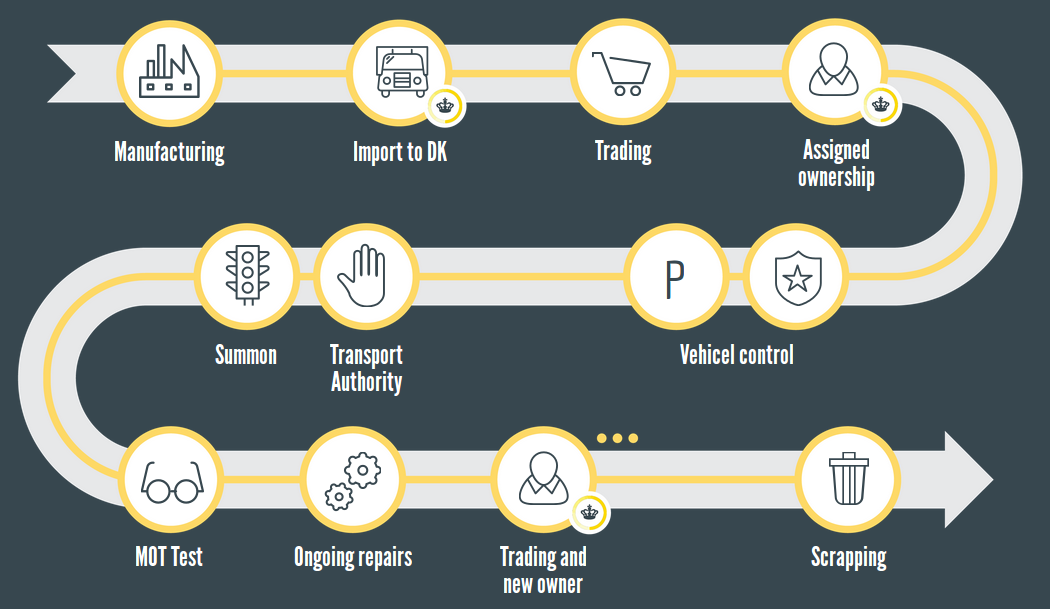
\includegraphics[width=\textwidth]{lifecycle.png}
  \caption{Vehicle life cycle}
  \label{fig:lifecycle}
\end{figure}

\section{Vehicle taxation in Denmark}
Taxation-wise there are several places where the Tax Agency needs to
be involved. When a car is imported, it has to be registered and a
registration tax has to be paid, it does not matter whether the car is
new or used. A yearly ownership tax is also collected for car owners,
and the Tax Agency thus also needs to know when a car is sold. Also,
several fees can be levied as part of the process, for example a
re-registration fee. It is also the Tax Agency's job to make sure that
all registered cars are insured by their owner.

\section{Core challenges}
As outlined in the description above, the core challenges are:

\begin{itemize}
\item Giving buyer knowledge of vehicle history, which he can trust
\item Giving seller trust, that the buyer will not commit fraud, and
  use the vehicle in the sellers name.
\item Ensuring that ownership taxes are collected from the rightful
  owner of the vehicle
\end{itemize}


\chapter{Trading contracts}
\label{sec:trading}
Now let us look at how blockchain systems can help mitigate the issues
of the Danish Motor Registry. As described in Section \ref{sec:case},
the main underlying challenge is the transfer of ownership between a
seller and a buyer. This ownership is represented by a contract, a so
called \emph{Certificate of Title} or in the case of a vehicles, a
\emph{Vehicle Title}. Trading a vehicle, thus really means trading the
Vehicle Title, stating who is the rightful owner. In this section we
will describe the current process of such a trade, and we will
describe how a blockchain solution, can mitigate most of the current
problems.

\section{Trading vehicles today}
The current process of trading a car between two persons
(private-to-private), is as follows:

\begin{enumerate}
\item Buyer inspects the condition of the car
\item Seller and buyer agrees on a price
\item Seller hands the registration certificate to the buyer. Buyer
  transfers the agreed amount of money to the sellers bank account.
\item When the money is received, the seller hands the car keys to buyer.
\item The buyer goes to \url{http://motorregister.skat.dk} and
  re-registers the car in his name.
\end{enumerate}
This process is risky for on both the seller and the buyer.
\begin{itemize}
\item The seller must trust that the buyer performs Step 5. The seller
  risks that levies will continue to be collected from him, not the
  new owner. The seller also risks that the buyer uses the car illegal
  activities or is involved in accident while the car is still insured
  by the seller.
\item In Step 3, The buyer has no way to verify that the registration
  certificate is correct. There is a risk that there is hidden debt in
  the car, that the car is stolen or that the car has been through
  major repairs.
\end{itemize}

\section{Trading on the blockchain}
\label{sec:trading_on_blockchain}
We will now describe how a blockchain solution might solve these trust
issues between the seller and the buyer. When a blockchain is used,
the Vehicle Title might be stored as an \emph{updateable} contract
\emph{on} the blockchain. By doing this the blockchain network agrees
on this contract as valid and we can trust its content.

In addition to carrying information identifying the actual car, the
contract may also be updated with police reports, MOT test outcomes,
insurance information and so on, which the buyer might be interested
in.

When a contract changes hands, it changes hands immediately, and SKAT
as well as insurance companies are notified immediately. By making the
money transfer and the change of ownership in the contract part of the
same transaction, we also protect the seller from the risks described
above. The fact that a new owner is recorded in the contract, is what
counts as re-registration. No additional re-registration is
necessary.

We have illustrated the transaction process of trading a vehicle using
the blockchain in Figure \ref{fig:shift-of-ownership}.

\begin{figure}
  \centering
  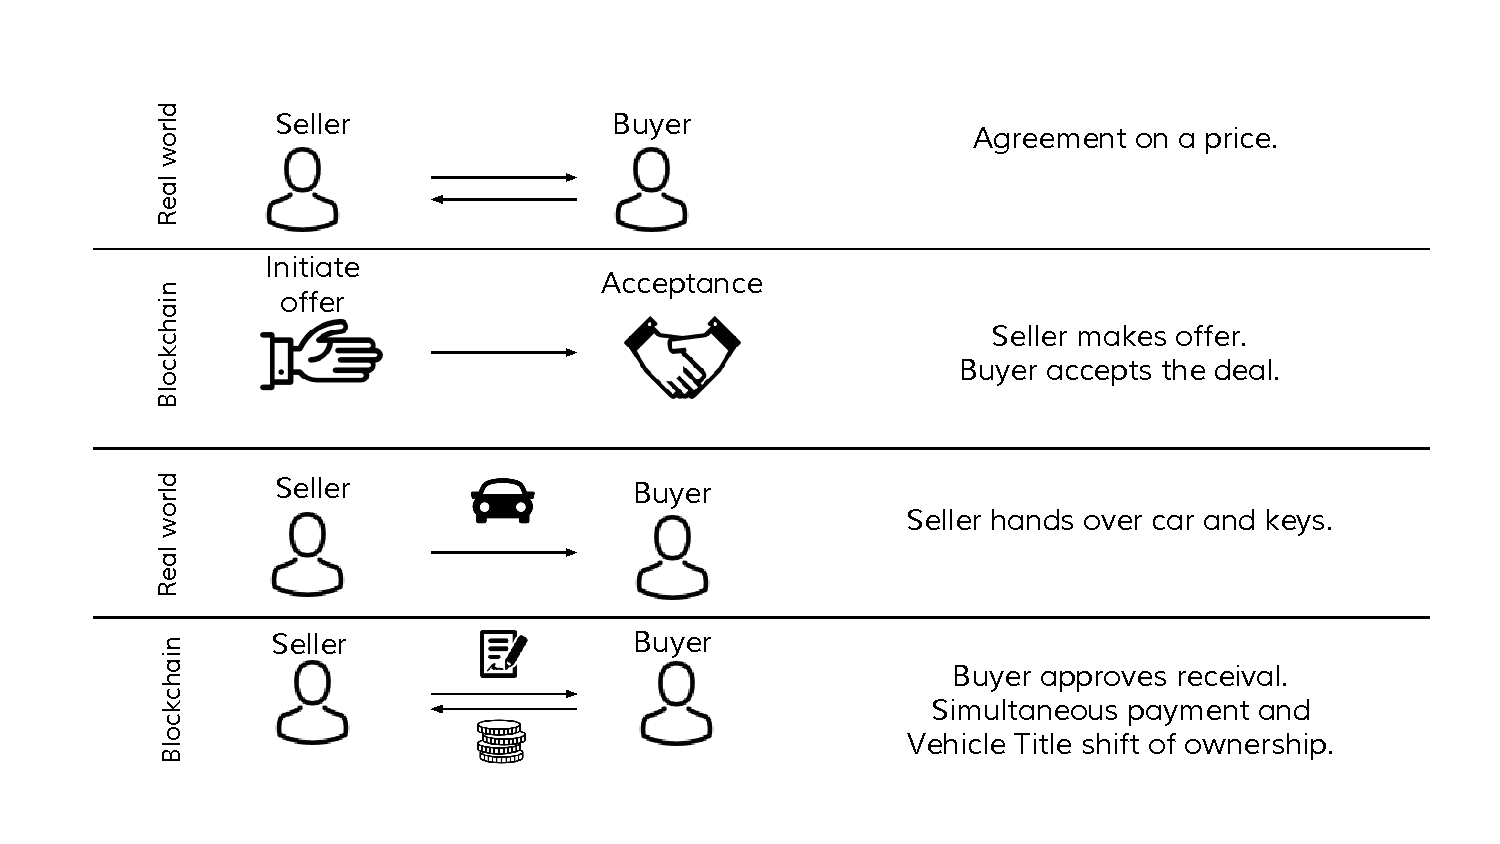
\includegraphics[width=\textwidth]{shift-of-ownership.pdf}
  \caption{Transaction process for shift of ownership.}
  \label{fig:shift-of-ownership}
\end{figure}

The initial contract will be created by the car factory, and at every
step through the supply-chain the car will be traded, and ownership
updated. Alternatively, we can wait and only associate contracts with
cars as soon as they enter the country, and limit whom may issue new
Vehicle Titles to SKAT or MOT test centers.

The problems described here are not only found in trades involving
cars. The same type of risks arise when selling or buying a house. In
fact, this blockchain scheme can be generalised, and we can build a
general framework for trading \textit{any} contract that can be
represented on the blockchain. We present such a framework implemented
in Ethereum in Section \ref{sec:implementation}.

% \todo{trading secrets, e.g. a private key}
% \todo{Certcoin https://eprint.iacr.org/2014/803.pdf}

\section{Identifying physical objects}
In a property registry it is crucial that properties are completely
identifiable. This is usually also done using a trusted third-party as
well as tagging the object, for example through a serial number
(e.g. Vehicle Identification Number). In a blockchain solution, such a
serial number might be added as an electronic tag. However, just as
with ordinary serial numbers, such a tag might be tampered with and
disputes might still need to be settled outside the blockchain in such
situtations. MOT test sites might constitute the trusted third party,
who verifies such tags every few years.

\section{User authentication}
Just as essential as identifying the physical object mentioned in
contract, is associating information about the actual human owner of
the property. 

In the Bitcoin system, it is often seen as a feature that users are
not authenticated. Coins are associated with a wallet address (a hash
of the public-key in a public/private keypair). If you loose the
keypair associated with that wallet address, you essentially loose the
coins associated with it, and they can never be reclaimed.

To authenticate users, a trusted third party is again necessary. In
Denmark NemID might be used (governmental digital identification
system). Alternatively, a system such as
Keybase\footnote{https://keybase.io/} might be used, where users prove
their identity through Social media accounts (e.g. by posting a key in
a Twitter message).

\chapter{Representing non-crypto currencies}
\label{sec:currency}
An orthogonal issue, to the issue of trading contracts, is the
question of how non-crypto currencies, like Euro or Danish Kroner
(DKK) should be represented on a blockchain. We want to support trades
which are not settled in Bitcoin or Ether, but on our current
financial markets. One approach is to go through an exchange and
exchange Euro or DKK for Ether whenever a sale is performed, this
however incurs overhead of exchange rates and potential fees.

Another possibility is to represent these currencies as
\textit{tokens} on Ethereum. In Ethereum the concept of token is a
standardized way to represent coins, or other fungible goods, such as
representing membership. In Ethereum it is implemented as a single
contract which manages a list of who owns which token.

With such a token contract we could make 1 token equal to 1 Øre (0.01
Kroner), and users should then be able to trade in actual danish
kroner for such tokens. To do this, we have to assume that a trusted
third-party will allow such a conversion back and forth between Danish
Kroner and block-chain tokens. This third-party could be the Danish
Central Bank or a major privately owned bank. Currently most
transactions are already only represented digitally, and such a
conversion will thus be a matter of conversion from the current
database-representation to a blockchain
\emph{token}-representation. In the rest of the paper we assume that
such a trusted third-party exists, and we use tokens as currency when
trading contracts.

\chapter{Implementation}
\label{sec:implementation}
As mentioned in the end of Section \ref{sec:trading_on_blockchain},
the vehicle trading problem can be generalised to trading any contract
on the blockchain. We have implemented a prototype allowing such
trades through a user selected intermediary which is also represented
as a contract. Each intermediary is specialised to holding values of a
certain currency (a certain token type).

To create a tradeable contract, the user creates a contract deriving
from the contract \texttt{BaseTradeable} shown in Figure
\ref{fig:tradeable}, and extends it with its own logic. In our case we
could create a contract \texttt{VehicleTitle} which extends on
\texttt{BaseTradeable} by also registering the Vehicle Identification
Number (VIN), the registration number (number plates), accident
history, owner history and so on, as well as allowing the various
parties (e.g. insurance company) to update the contract when new
information is available.

If we want \emph{all} car sales to go through the Danish Motor
Registry, we could create a special intermediary-contract, as the sole
allowed intermediary when selling cars registered in Denmark. This
requirement would thus be part of the contract
\texttt{VehicleTitle}. However, an alternative approach is to allow
any contract to listen for the event that a car has been sold. In this
way the taxation authority can step back, and only monitor all
\texttt{VehicleTransfer} events, without being an involved participant
in car sales. When they need to levy ownership taxes, they can look up
in their database in see exactly who owned which vehicle when.

\begin{figure}
%\todo{add VehicleTransfer event}
\begin{lstlisting}
contract BaseTradeable {
  address owner;
  address intermediary = 0;
  address receiver     = 0;

  function BaseTradeable () {
    owner = msg.sender;
  }

  // Issue an offer through a given intermediary  
  function makeOffer (address _intermediary,
                      address buyer, uint256 amount)
  only(owner) notForSale {
    Intermediary i = Intermediary(intermediary);
    intermediary = _intermediary;
    receiver = buyer;
    i.receiveOffer(this, owner, buyer, amount);
  }

  // Called by intermediary if the sale i cancelled
  function saleCancelled () only(intermediary) forSale {
    intermediary = 0;
    receiver = 0;
  }
  // Called by intermediary to transfer ownership
  function transferContract () only(intermediary) {
    owner = receiver;
  }
  ...
}
\end{lstlisting}

\caption{Tradeable contract (modifiers not shown)}
\label{fig:tradeable}
\end{figure}

\begin{figure}
  \begin{lstlisting}
contract Intermediary {
  // Select token-currency on creation
  function Intermediary(Token currency) {  }

  // Seller makes an offer to a buyer
  function receiveOffer(address theContract, address seller,
                        address buyer, uint256 amount) only(buyer) { }

  // Buyer approves by transferring funds to the intermediary.
  function receiveApproval(address from, uint256 value,
                           address token, address theContract) only(from) {}

  // Seller revokes an offer.
  // If the buyer has paid, his money is transferred back
  function revokeOffer(address theContract) isSellerOf(theContract) {}
  
  // Buyer approves. Goods are received.
  function completeTransaction(address theContract) isBuyerOf(theContract) {}

  // Buyer aborts the transaction. Goods are not received
  function abortTransaction(address theContract) isBuyerOf(theContract) {}
}
  \end{lstlisting}
  \caption{Intermediary interface}
  \label{fig:intermediary}
\end{figure}

\chapter{Experience using Ethereum}
\label{sec:ethereum-experiences}
As mentioned, we used the Ethereum platform for building this
prototype. We want to report on our experiences using the platform,
and whether continued development of a new Danish Motor Registry on
Ethereum is worthwhile. 

From a user perspective the Ethereum blockchain and wallet application
are easy to install and easy to use for trading Ether. However, as a
developer, the platform still has many shortcomings. The documentation
of both Solidity language and the App-development frameworks Truffle
and Embark are seriously lacking. Good testing and debugging tools are
missing and the Solidity compilers error messages are poor.

Another aspect entirely is the language Solidity. Solidity is based on
object-oriented principles, and in many ways seems inspired by
JavaScript. This makes contracts and transactions hard to reason
about. Transaction logic might be split between multiple contract
objects, and what would constitute a single contract on paper might be
spread across multiple contract objects in Solidity. Contracts whether
written in natural language or digital code should be easy to
comprehend, and easy to verify. For example, it is necessary to verify
that no transaction history can provoke an ill-defined state.

% Here are some of the problems, anti-patterns and weird design
% decisions we encountered using Solidity:
% \begin{itemize}
% \item Exceptions does not carry a reason. All exceptions look the same.
% \item You can not catch exceptions.
% \item A special noname function is needed \texttt{function () \{ throw; \}} to return funds
% \item Modifiers needs a \texttt{\_} character. This is not checked by
%   the compiler. A runtime error occurs.
% \item A method accepting an instance of class C, must still be casted
%   to class C before use (see the first line in the function
%   \texttt{makeOffer}, Figure \ref{fig:tradeable})
% \item Class-dependencies can be cyclic, but only if your classes are
%   all in the same file.
% \end{itemize}
Eventually a better language than Solidity may be introduced, or
Solidity might improve over time. A framework for formal verification
of Solidity programs has been presented, where users can prove various
properties about contracts \cite{bhargavanshort}. 

Research in alternative contract languages is ongoing, and have been a
topic in programming language research even before blockchains was
brought to the table. Using certified contract languages, such as
\cite{hvitved2011contract} for ERP systems or \cite{bahr2015certified}
for financial contracts, the compiler can help us limit the contract
we can write (e.g. to avoid runtime errors), analyse our contracts for
correctness, automatically assign blame when a party does not follow
the contract and do automatic risk-analysis and pricing of financial
contracts.

In short, our conclusion is that Ethereum currently is not a stable
enough platform for anything except prototypes. Ethereum is still are
young project, and better development tools and contract languages
will hopefully arrive.

% \chapter{User experience design}
% SKAT provided us with a complete prototype of the user interface in an
% app used for private-private car sales. We will not go into more
% detail with that here, but just refer the reader to try it out here:
% \url{}

% In addition to the steps necessary for trading a car between two
% private parties, it is also int

% \todo{Describe participants/actors: who are the users?}

% \todo{Contracts should be tied to NemID or Corporate ID.}

% \todo{Describe the entire process suggested in Mockup-app from SKAT.}

% \todo{IoT, Immobilisers in cars}

% \todo{users should trust blockchain technology, as the actual
%   contracts are now on the blockchain}

\chapter{Future work}
\label{sec:futurework}
Further questions remain to be answered before a blockchain system for
the Danish Motor Registry can be implemented.  First and foremost, the
reasons for choosing a blockchain system must be exactly
clear. Several design choices can be made, and to decide more
knowledge about the motivation for abandoning traditional systems are
necessary.

A blockchain solution might be run publicly or privately, but when run
privately it is in essence ``just'' another kind of shared
database. Running a private blockchain might still make sense if a lot
of parties, or competing parties, needs to agree on the same history
of events. There however has to be a trust issue between the parties,
otherwise solutions based on regular distributed databases might be
more appropriate (e.g. federated databases, replicated logs). 

We need to understand the privacy requirements and how the different
parties interact with the Motor Registry, to decide between a public
blockchain (such as Ethereum), a privately run blockchain, a
traditional centralized system using some kind of distributed database
architecture. Another alternative is a public blockchain, but where
public-key encryption is used to hide confidential information. In
this way mining can be done by outsiders, while keeping the
information secure.

Using a blockchain solution depending on the resource wasteful
Proof-of-Work scheme will probably not create positive headlines for
the Danish Tax Agency. If a privately run blockchain is chosen, a
Proof-of-Stake system might be worthwhile, but further experience with
alternative consensus mechanisms is necessary.

Any IT system will need to be updated over time as new legislation and
new products arise. The question of how a blockchain system can be
updated is thus pertinent. For example, how could we add a new type
information to all existing Vehicle Title contracts, or incorporate a
new rule that in some way limits the sales of vehicles. This needs to
be considered before such a system is implemented, as old contracts on
the blockchain might need to have a built-in ``upgrade''-routine.

Another aspect is how much data should really be stored on the
blockchain. Storage in Ethereum is costly, as this increases the
transaction costs, thus with the current model, it would probably be
better to store larger files (e.g. photos of cars) off chain,
e.g. using a peer-to-peer system such as IPFS.

As mentioned in Section \ref{sec:ethereum-experiences} it would also
be interesting to see whether we could express the same logic in a
more secure contract language like CSL \cite{hvitved2011contract}, and
how such a contract language can be compiled to Ethereum bytecode.

Many cars today are already produced with a so called
\textit{immobiliser}, which prevents the engine from running without
the correct key present. Such keys could be digitised and stored as
part of the contract on the blockchain.

\chapter{Conclusion}
\label{sec:conclusion}
Blockchain technology is in early stage development, many questions
still needs further research, before large scale systems are
built. Especially two areas the community has not settled for a
standard practice: consensus mechanisms and contract programming
languages. The future will tell which mechanisms and languages will
win, further research might be necessary.

Blockchain technology is however already used for certain Certificate
of Title registries. Two examples are the
Bitland\footnote{http://bitlandglobal.com/} which tracks land and
property ownership in Ghana and
Everledger\footnote{http://everledger.io/}, which tracks diamond
ownership.

\bibliographystyle{plainurl}
\bibliography{bibliography}



\end{document}